%-----------------------------------------------------------------------------------------------------------%
\newpage

\def \Session {1}
\setcounter{chapter}{\Session-1}

\part{پیشنیاز های ریاضی}

{
    \Large
    \begin{spacing}{1.5}
        بازی های ویدیویی سعی در شبیه سازی دنیای مجازی دارند.
        با این حال، کامپیوترها، به دلیل ماهیت خود، اعداد را محاسبه می کنند. بنابراین مشکل چگونگی انتقال یک جهان به یک کامپیوتر مطرح می شود.
        پاسخ این مشکل میتواند اینگونه باشد که جهان‌های ما و فعل و انفعالات موجود در آن را کاملاً ریاضی توصیف کنیم.
        در نتیجه، ریاضیات نقش اساسی در توسعه بازی های ویدیویی ایفا می کند.

        در این بخش، ابزارهای ریاضی که در این کتاب مورد استفاده قرار گرفته اند، معرفی می کنیم. تأکید ما بر بردارها، سیستم های مختصات، ماتریس ها و تبدیل ها است، زیرا این ابزارها تقریباً در همه ی برنامه های نمونه این کتاب استفاده شده اند.
        علاوه بر توضیحات ریاضی، بررسی و نمایش کلاس ها و توابع مربوطه از کتابخانه ریاضی DirectX را نیز ارائه میکنیم.

        توجه داشته باشید که موضوعاتی که در اینجا مورد بررسی قرار می‌گیرند، تنها مواردی هستند که برای درک ادامه ی این کتاب ضروری اند.
        این کتاب به هیچ وجه راه حل جامعی برای ریاضیات بازی های ویدیویی نیست.

    \end{spacing}

    \begin{theo}{thm:pythagoras}
        \Large
        برای خوانندگانی که مایل به ارجاع کامل تر به ریاضیات بازی های ویدیویی هستند، کتاب های زیر را توصیه می کنیم.
        \lr{
            \begin{enumerate}
                \item {Essential Mathematics for Games and Interactive Applications: A Programmer's Guide (Verth04)}
                \item {Mathematics for 3D Game Programming and Computer Graphics (Lengyel02)}
            \end{enumerate}
        }
    \end{theo}
}
\newpage
{
    \Large
    \begin{spacing}{1.5}
        \textbf{فصل 1، جبر برداری:} بردارها اساسی ترین اشیاء ریاضی مورد استفاده در بازی های کامپیوتری هستند.
        ما از بردارها برای نشان دادن موقعیت ها، جابجایی ها، جهت ها، سرعت ها و نیروها استفاده می کنیم.
        در این فصل، بردارها و عملیات مورد استفاده برای کار با آنها را مطالعه می کنیم.

        \textbf{فصل 2، جبر ماتریسی:} ماتریس ها روشی کارآمد و فشرده برای نمایش تبدیل ها ارائه می دهند.
        در این فصل با ماتریس ها و عملیات تعریف شده بر روی آنها آشنا می شویم.

        \textbf{فصل 3، تبدیل:} این فصل سه تبدیل هندسی اساسی را بررسی می کند: مقیاس بندی، چرخش و انتقال.
        ما از این تبدیل ها برای کار با اشیاء سه بعدی در فضا استفاده می کنیم.
        علاوه بر این، تغییر تبدیل مختصات را توضیح می دهیم، که برای تبدیل مختصات هندسی از یک سیستم مختصات به سیستم دیگر استفاده می شود.
    \end{spacing}
}

%-----------------------------------------------------------------------------------------------------------%
\newpage

\chapter{جبر برداری}

{
    \Large
    \begin{spacing}{1.5}
        بردارها نقش مهمی در گرافیک کامپیوتری، تشخیص برخورد و شبیه سازی فیزیکی ایفا می کنند که همگی اجزای رایج در بازی های ویدئویی مدرن هستند.
        رویکرد ما در اینجا غیر تخصصی و عملی است به همین دلیل پیشنهاد ما کتاب \lr{Verth04} (در نکته ی قبل ذکر شده است) است که کتابی اختصاصی برای ریاضیات بازی های سه بعدی/گرافیک است.
        ما بر اهمیت بردارها بسیار تأکید داریم زیرا در بیشتر برنامه های آزمایشی این کتاب استفاده شده اند.

        \textbf{اهداف:}

        \begin{enumerate}
            \item {یادگیری نحوه نمایش بردارها به صورت هندسی و عددی}
            \item {یادگیری عملیات تعریف شده بر روی بردارها و کاربردهای هندسی آنها}
            \item {آشنایی با توابع برداری و کلاس های کتابخانه \lr{DirectXMath}}
        \end{enumerate}
    \end{spacing}
}
\newpage
{
    \textbf{\BTitr بردار ها:}

    \Large
    \begin{spacing}{1.5}
        بردار به کمیتی اشاره دارد که هم اندازه و هم جهت دارد.
        به کمیت هایی که هم اندازه و هم جهت دارند، کمیت های بردار می گویند.
        نمونه‌هایی از کمیت‌های برداری عبارتند از نیروها (نیرو در جهت خاصی با قدرت/اندازه معین اعمال می‌شود)، جابه‌جایی (جهت برآیند و فاصله حرکت ذره)، و سرعت‌ها (سرعت و جهت).
        بنابراین، بردارها برای نمایش نیروها، جابجایی ها و سرعت ها استفاده می شوند.
        علاوه بر این، ما همچنین از بردارها برای تعیین جهات خالص استفاده می کنیم،
        مانند جهتی که بازیکن در یک بازی سه بعدی به آن نگاه میکند،
        جهتی که یک چند ضلعی رو به آن قرار دارد، جهتی که پرتوی نور در آن حرکت می کند،
        یا جهتی که در آن یک پرتو نور از یک سطح منعکس می شود.

        اولین مرحله در توصیف ریاضی بردار ، توصیف هندسی آن است: ما به صورت گرافیکی یک بردار را با یک پاره خط جهت دار مشخص می کنیم (شکل \ref{fig:4.Session.1.1.1})، که در آن طول نشان دهنده بزرگی بردار و سر کمان نشان دهنده جهت بردار است.
        به این نکته باید توجه داشته باشیم که مکانی که در آن یک بردار رسم می‌کنیم بی‌اهمیت است، زیرا تغییر مکان، بزرگی یا جهت را تغییر نمی‌دهد (دو ویژگی که یک بردار دارد).
        بنابراین می گوییم دو بردار برابر هستند اگر و تنها اگر طول یکسانی داشته باشند و در یک جهت باشند.
        بنابراین، بردارهای \lr{u} و \lr{v} ترسیم شده در قسمت آ شکل \ref{fig:4.Session.1.1.1} در واقع برابر هستند زیرا طول و جهت یکسانی دارند.
        در واقع، چون مکان برای بردارها اهمیتی ندارد، ما همیشه می‌توانیم یک بردار را بدون تغییر هویت آن ، انتقال دهیم (زیرا انتقال نه طول و نه جهت را تغییر می‌دهد).
        توجه داشته باشید که ما می‌توانیم \lr{u} را طوری انتقال دهیم که کاملاً بر \lr{v} همپوشانی داشته باشد (و بالعکس) و در نتیجه آنها را غیرقابل تشخیص کنیم. این نیز دلیلی برای برابری آنهاست.

        \begin{figure}[H]
            \centering
            \setlength{\belowcaptionskip}{-10pt}
            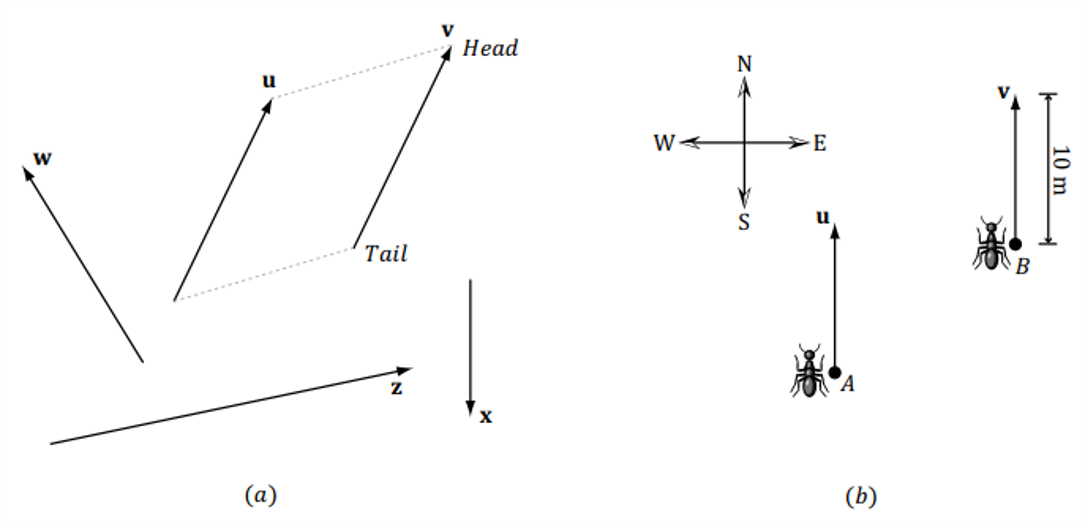
\includegraphics[width=\textwidth]{Images/4/4.Session.1.1.1}
            \caption{(الف) بردار هایی که روی صفحه ی دوبعدی کشیده شده اند.
                (ب) بردار هایی که مورچه ها را برای حرکت 10 متر در جهت شمال راهنمایی میکنند.}
            \label{fig:4.Session.1.1.1}
        \end{figure}

        به عنوان یک مثال فیزیکی، بردارهای \lr{u} و \lr{v} در قسمت ب شکل \ref{fig:4.Session.1.1.1} هر دو به مورچه ها میگویند در دو نقطه مختلف \lr{A} و \lr{B} ده متر به سمت شمال حرکت کنند.
        دوباره \lr{u = v} را داریم.
        بردارها خود مستقل از موقعیت هستند و
        آنها به سادگی به مورچه ها آموزش می دهند که چگونه از جایی که هستند، ده متر (طول) به سمت شمال (جهت) حرکت کنند.
    \end{spacing}
}

{
    \textbf{\BTitr بردارها و سیستم های مختصات:}

    \Large
    \begin{spacing}{1.5}
        اکنون می‌توانیم عملیات هندسی مفیدی را روی بردارها تعریف کنیم، که سپس می‌توان از آنها برای حل مسائل مربوط به کمیت‌های برداری استفاده کرد.
        با این حال، از آنجایی که کامپیوتر نمی تواند با بردارها به صورت هندسی کار کند، باید راهی برای تعیین عددی بردارها پیدا کنیم.
        بنابراین یک سیستم مختصات سه بعدی را در فضا معرفی می کنیم و همه بردارها را طوری انتقال میدهیم که دم آن ها با مبدا منطبق باشد (شکل \ref{fig:4.Session.1.1.2}).
        سپس می‌توانیم یک بردار را با تعیین مختصات سر آن شناسایی کنیم و مانند شکل \ref{fig:4.Session.1.1.3}، \lr{v = (x, y, z)} را بنویسیم.
        اکنون می توانیم یک بردار را با سه \lr{float} در یک برنامه کامپیوتری نشان دهیم.

        \begin{theo}{thm:pythagoras}
            \Large
            اگر به صورت دو بعدی کار کنیم، فقط از یک سیستم مختصات دو بعدی استفاده می کنیم و بردار فقط دو مختصات دارد:
            \lr{v = (x, y)} و می توانیم یک بردار را با دو \lr{float} در یک برنامه کامپیوتری نشان دهیم.
        \end{theo}

        \begin{figure}[H]
            \centering
            \setlength{\belowcaptionskip}{-10pt}
            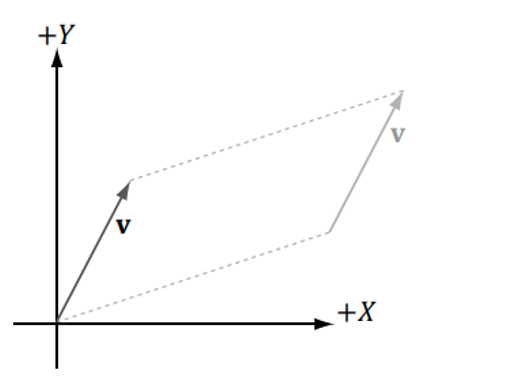
\includegraphics[width=0.5\textwidth]{Images/4/4.Session.1.1.2}
            \caption{\lr{v} را طوری انتقال میدهیم که دم آن با مبدأ سیستم مختصات منطبق
            باشد. وقتی دم یک بردار با مبدا منطبق می شود، می گوییم که در موقعیت استاندارد قرار دارد.}
            \label{fig:4.Session.1.1.2}
        \end{figure}

        \begin{figure}[H]
            \centering
            \setlength{\belowcaptionskip}{-10pt}
            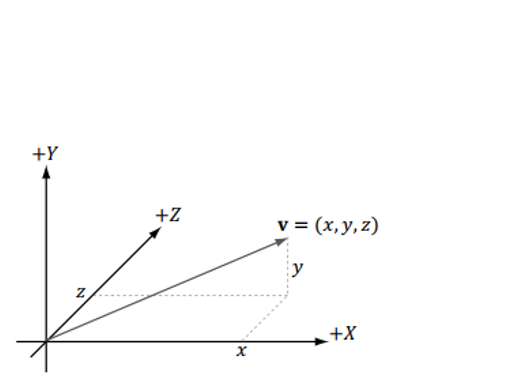
\includegraphics[width=0.5\textwidth]{Images/4/4.Session.1.1.3}
            \caption{یک بردار مشخص شده توسط مختصات نسبت به یک سیستم مختصات.}
            \label{fig:4.Session.1.1.3}
        \end{figure}

        شکل \ref{fig:4.Session.1.1.4} را در نظر بگیرید که یک بردار \lr{v} و دو فریم (\lr{frame}) در فضا را نشان می دهد. (توجه داشته باشید که ما از اصطلاحات فریم، فریم مرجع، فضا و سیستم مختصات استفاده می کنیم که همگی در این کتاب به یک معنا هستند.)
        می توانیم \lr{v} را طوری انتقال دهیم که در هر یک از دو سیستم مختصات در موقعیت استاندارد قرار گیرد. با این حال، مشاهده کنید که مختصات بردار \lr{v} نسبت به سیستم مختصات \lr{A} با مختصات بردار \lr{v} نسبت به سیستم مختصات \lr{B} متفاوت است.
        به عبارت دیگر، همان بردار \lr{v} نمایش مختصاتی متفاوتی برای سیستم مختصات های متمایز دارد.

        \begin{figure}[H]
            \centering
            \setlength{\belowcaptionskip}{-10pt}
            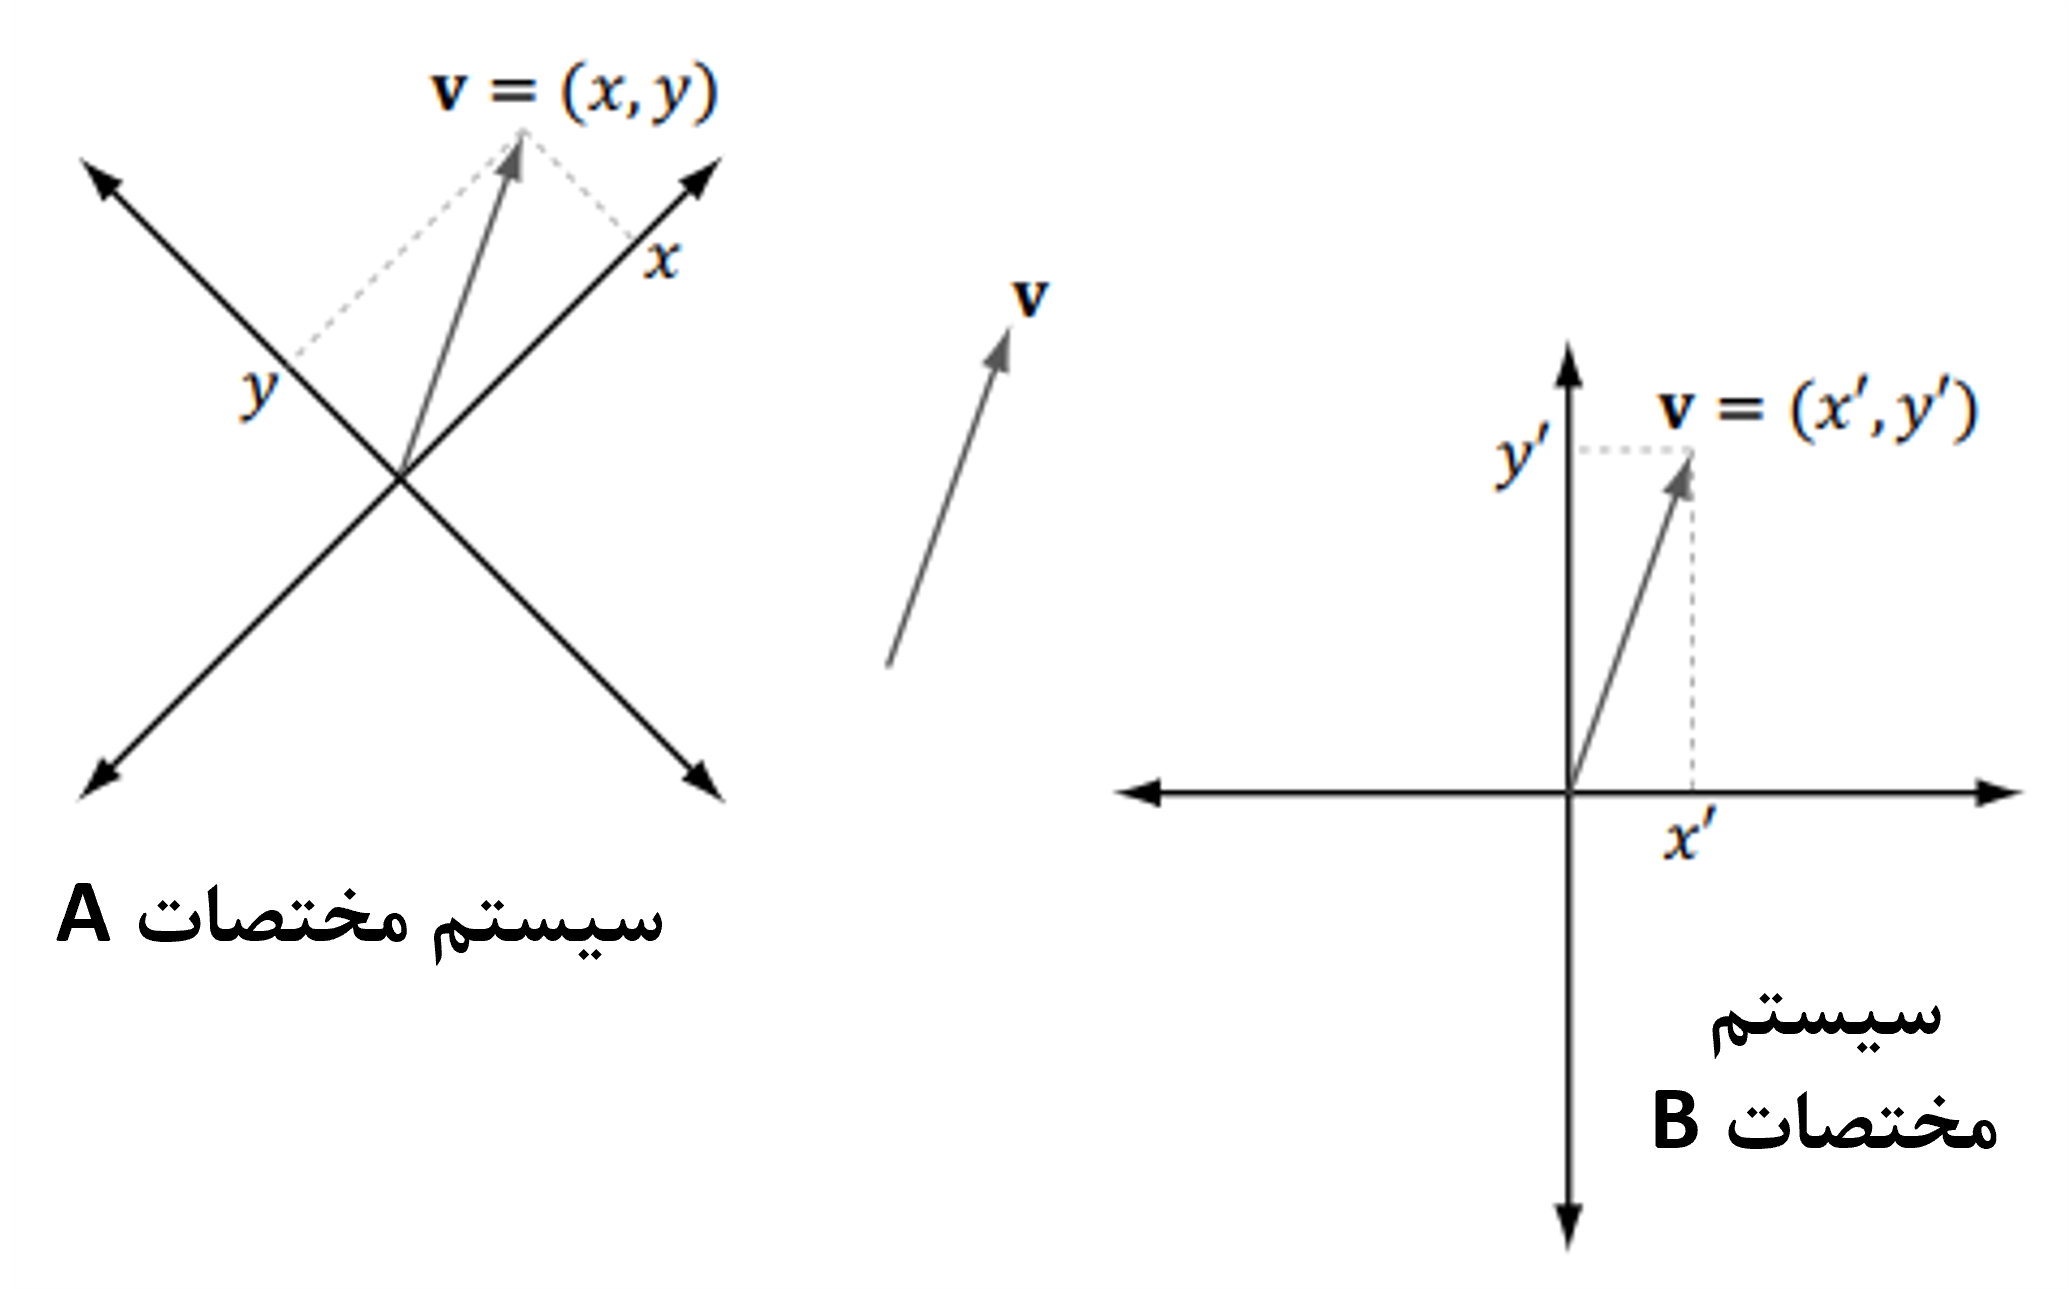
\includegraphics[scale=0.7]{Images/4/4.Session.1.1.4}
            \caption{همان بردار v زمانی که نسبت به سیستم مختصات های مختلف تعریف شود، مختصات متفاوتی دارد.}
            \label{fig:4.Session.1.1.4}
        \end{figure}

        این ایده شبیه به مثال دما است. آب در 100 درجه سانتیگراد یا 212 درجه فارنهایت می جوشد.
        دمای فیزیکی آب جوش بدون توجه به مقیاس یکسان است (یعنی نمی‌توانیم نقطه جوش را با انتخاب مقیاس متفاوت کاهش دهیم)،
        اما بر اساس مقیاسی که استفاده می‌کنیم عدد اسکالر متفاوتی را به دما اختصاص می‌دهیم.
        به طور مشابه، برای یک بردار، جهت و بزرگی آن، که در پاره خط جهت دار تعبیه شده است، تغییر نمی کند.
        فقط مختصات آن بر اساس سیستم مختصات که برای توصیف آن استفاده می کنیم تغییر می کند.
        این نکته ی مهمی ست زیرا به این معنی است که هرگاه یک بردار را با مختصات شناسایی کنیم، آن مختصات نسبت به برخی از سیستم های مختصات هستند.
        اغلب در گرافیک های کامپیوتری سه بعدی، از بیش از یک سیستم مختصات استفاده می کنیم و بنابراین، باید شناسایی کنیم که مختصات یک بردار نسبت به کدام سیستم مختصات است.
        علاوه بر این، ما باید بدانیم که چگونه مختصات برداری را از یک سیستم مختصات به سیستم مختصات دیگر تبدیل کنیم.

        \begin{theo}{thm:pythagoras}
            \Large
            مشاهده میکنیم که بردارها و نقاط را می توان با مختصات (\lr{x, y, z}) نسبت به یک سیستم مختصات توصیف کرد.
            با این حال، بردارها و نقاط یکسان نیستند؛ یک نقطه نشان دهنده یک مکان در 3 فاصله است، در حالی که یک بردار نشان دهنده یک اندازه و جهت است.
        \end{theo}
    \end{spacing}
}

{
    \textbf{سیستم\BTitr  های مختصات چپگرد در مقابل راستگرد}

    \Large
    \begin{spacing}{1.5}
        \lr{Direct3D} از یک سیستم مختصات چپگرد استفاده می کند.
        اگر دست چپ خود را به صورتی بگیرید که انگشتان خود را به سمت محور x مثبت گرفته و سپس انگشتان خود را به سمت محور y مثبت خم کنید، انگشت شست شما در جهت محور z مثبت قرار می گیرد.
        شکل \ref{fig:4.Session.1.1.5} تفاوت بین یک سیستم مختصات چپ دست و راست دست را نشان می دهد.
        توجه کنید که در سیستم مختصات راستگرد، اگر دست راست خود را به صورتی بگیرید که انگشتان خود را به سمت محور x مثبت گرفته و سپس انگشتان خود را به سمت محور y مثبت خم کنید، انگشت شست شما در جهت محور z مثبت اشاره می کند.

        \begin{figure}[H]
            \centering
            \setlength{\belowcaptionskip}{-10pt}
            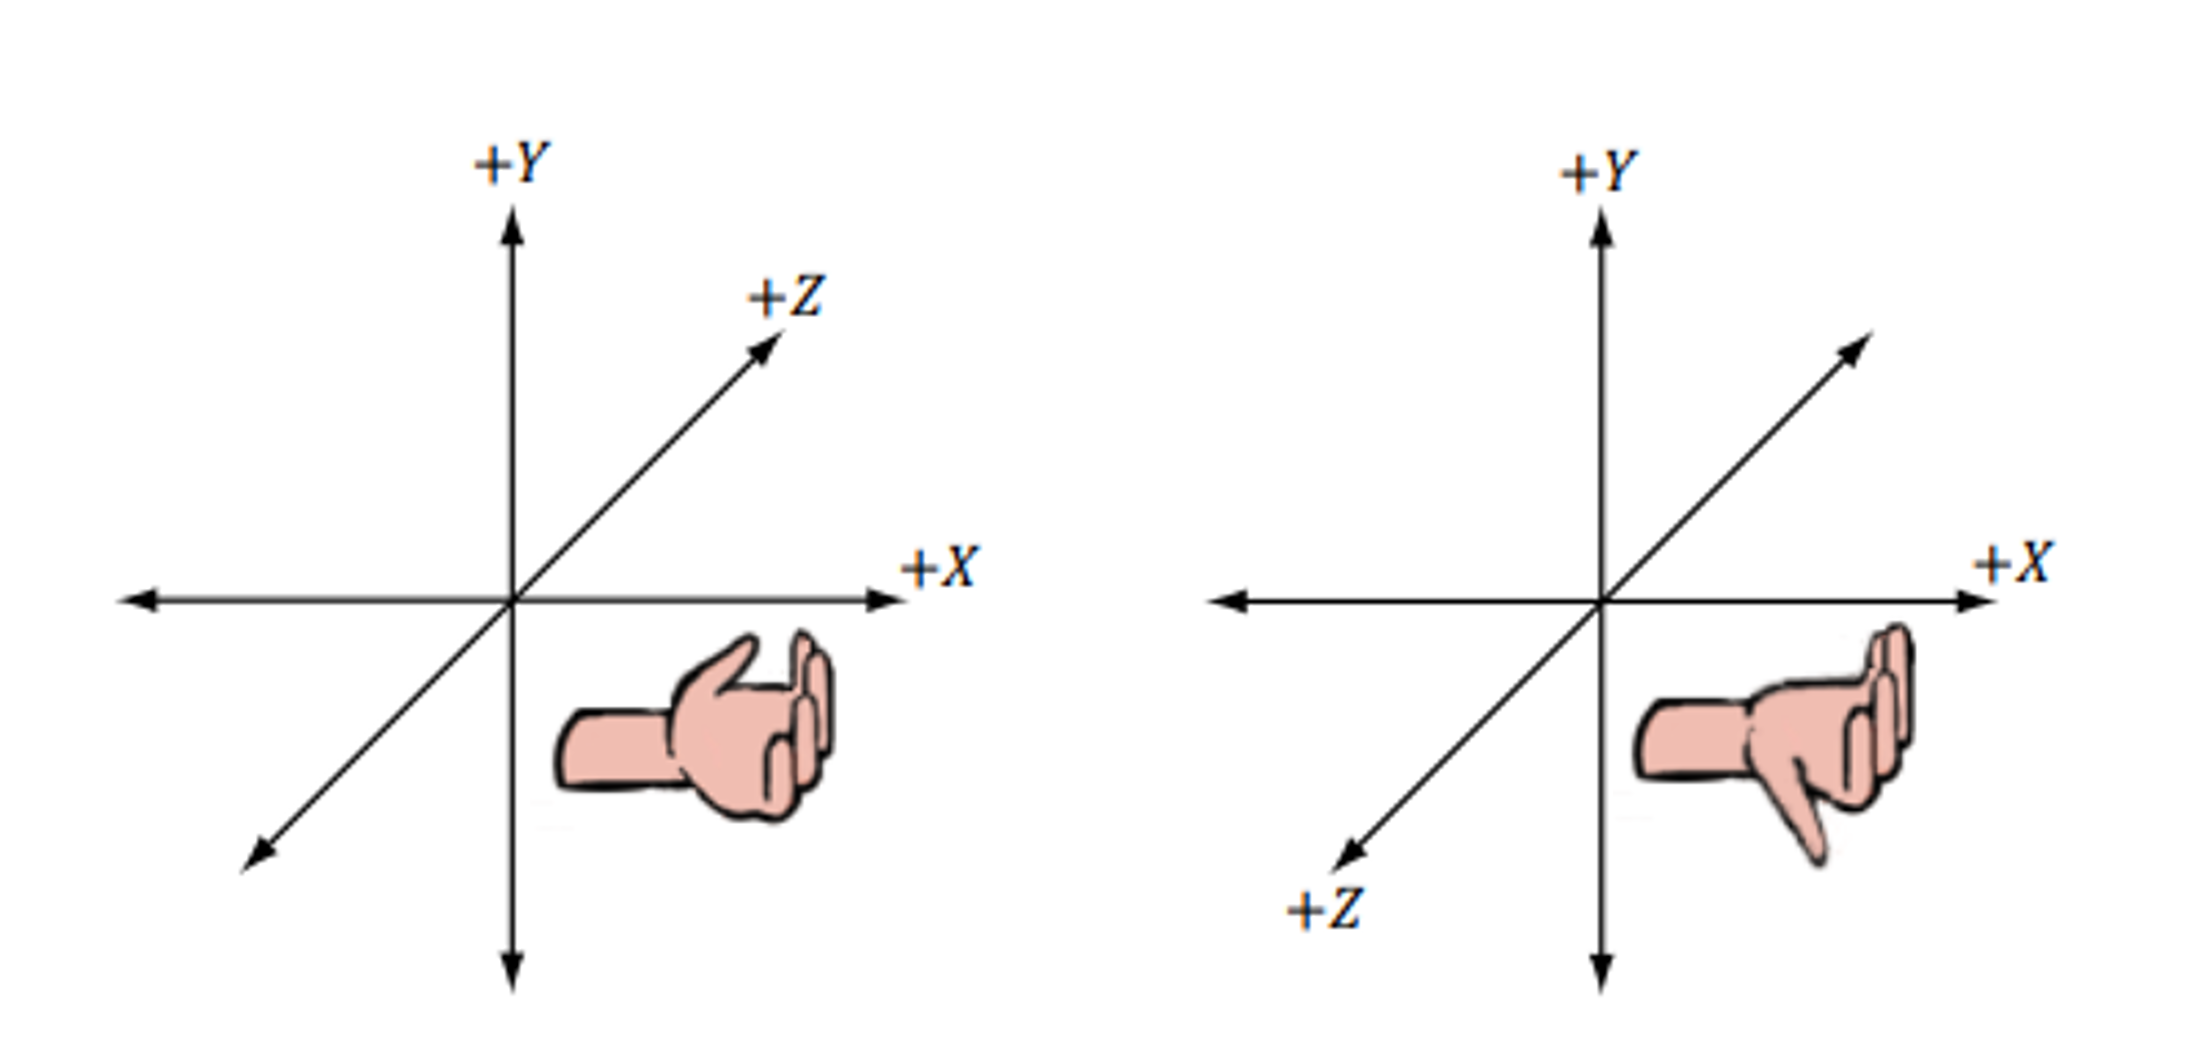
\includegraphics[scale=0.7]{Images/4/4.Session.1.1.5}
            \caption{در سمت چپ ما یک سیستم مختصات چپگرد داریم که محور z مثبت وارد صفحه می شود. در سمت راست ما یک سیستم مختصات راستگرد داریم که محور z مثبت از صفحه خارج می شود.}
            \label{fig:4.Session.1.1.5}
        \end{figure}
    \end{spacing}
}

{
    \textbf{\BTitr عملیات بردار پایه}

    \Large
    \begin{spacing}{1.5}
        اکنون با استفاده از نمایش مختصاتی، تساوی، جمع، ضرب اسکالر و تفریق را بر روی بردارها تعریف می کنیم.
        برای این چهار تعریف، فرض میکنیم $\textbf{u}=(u_{x},u_{y},u_{z})$ و  $\textbf{v}=(v_{x},v_{y},v_{z})$.

        \begin{enumerate}
            \item {دو بردار مساوی هستند اگر و تنها اگر اجزای متناظر آنها با هم برابر باشند.
            یعنی $\textbf{u}=\textbf{v}$ اگر و تنها اگر $u_{x}=v_{x}$ ، $u_{y}=v_{y}$ و $u_{z}=v_{z}$}
            \item {بردارها را به صورت جزء اضافه می کنیم: $\textbf{u}+\textbf{v}=(u_{x}+v_{x},u_{y}+v_{y},u_{z}+v_{z})$.
            توجه داشته باشید که فقط اضافه کردن بردارهایی با همان بعد ، منطقی ست.}
            \item {می توانیم یک اسکالر (یعنی یک عدد حقیقی) و یک بردار را ضرب کنیم و نتیجه یک بردار خواهد بود.
            فرض کنید k یک اسکالر باشد، پس $k\textbf{u}=(ku_{x},ku_{y},ku_{z})$. به این ضرب اسکالر می گویند.}
            \item {ما تفریق را بر حسب جمع بردار و ضرب اسکالر انجام می دهیم.
            \\یعنی $\textbf{u}-\textbf{v}=\textbf{u}+(-1\cdot\textbf{v})=\textbf{u}+(-\textbf{v})=(u_{x}-v_{x},u_{y}-v_{y},u_{z}-v_{z})$}
        \end{enumerate}

        مثال***
        فرض کنید $\textbf{u}=(1,2,3), \textbf{v}=(1,2,3), \textbf{w}=(3,0,-2), k=2$
        \lr{
            \begin{enumerate}
                \item {$\textbf{u}+\textbf{w}=(1,2,3)+(3,0,-2)=(4,2,1)$;}
                \item {$\textbf{u}=\textbf{v}$}
                \item {$\textbf{u}-\textbf{v}=\textbf{u}+(-\textbf{v})=(1,2,3)+(-1,-2,-3)=(0,0,0)=\textbf{0}$;}
                \item {$k\textbf{w}=2(3,0,-2)=(6,0,-4)$}
            \end{enumerate}
        }
        تفاوتی که در مورد سوم هست ، یک بردار خاص به نام بردار صفر را نشان می دهد که همه اجزای آن صفر است و با \lr{\textbf{0}} نشان داده می شود.


        مثال***
        ما این مثال را با بردارهای دوبعدی برای ساده‌تر کردن کار توضیح می‌دهیم. ایده ها مانند فضای سه بعدی هستند، فقط با یک جزء کمتر ، به صورت دو بعدی کار می کنیم.

        \begin{enumerate}
            \item {فرض کنید $\textbf{v}=(2,1)$، $\textbf{v}$ و $-\frac{1}{2}\textbf{v}$ چگونه از نظر هندسی با هم مقایسه می شوند؟
            توجه داریم که $-\frac{1}{2}\textbf{v}=(-1,-\frac{1}{2})$.
            با ترسیم نمودار $\textbf{v}$ و $-\frac{1}{2}\textbf{v}$ (قسمت آ شکل \ref{fig:4.Session.1.1.6})،
            متوجه می‌شویم که $-\frac{1}{2}\textbf{v}$ در جهت مخالف $\textbf{v}$ است و طول آن $\frac{1}{2}\textbf{v}$ است.
            بنابراین، از نظر هندسی، منفی کردن یک بردار را می‌توان به صورت "برگرداندن" جهت آن،
            و ضرب اسکالر را می توان به عنوان مقیاس بندی طول یک بردار در نظر گرفت.}

            \item {فرض کنید $\textbf{u}=(2,\frac{1}{2})$ و $\textbf{v}=(1,2)$. پس $\textbf{u}+\textbf{v}=(3,\frac{5}{2})$ .
            قسمت ب شکل \ref{fig:4.Session.1.1.6} نشان می‌دهد که جمع بردار از نظر هندسی به چه معناست:
            ما $\textbf{u}$ را به‌طور موازی انتقال میدهیم تا دم آن با سر $\textbf{v}$ منطبق شود.
            پس بردار مجموع ، برداری است که از دم $\textbf{v}$ شروع شده و با سر $\textbf{u}$ منتقل شده ختم می‌شود.
                (اگر $\textbf{u}$ را ثابت نگه داریم و $\textbf{v}$ را طوری انتقال دهیم که دم آن با سر $\textbf{u}$ منطبق شود، همین نتیجه را می گیریم.
                در این حالت، $\textbf{u}+\textbf{v}$ برداری خواهد بود که از دم $\textbf{u}$ شروع شده و با سر $\textbf{v}$ منتقل شده ختم میشود.)
                توجه داشته باشید که قوانین جمع بردار در زمانی که نیروها را با هم جمع می کنیم تا نیروی برآیند را به وجود بیاوریم، با انتظار ما مطابقت دارد:
                اگر دو نیرو (بردار) را در یک راستا اضافه کنیم، نیروی برآیند قوی تری (بردار طولانی تر) در آن جهت دریافت می کنیم.
                اگر دو نیرو (بردار) مخالف یکدیگر را بهم اضافه کنیم، نیروی برآیند ضعیف تری (بردار کوتاه تر) به دست می آید.
                شکل \ref{fig:4.Session.1.1.7} این ایده ها را نشان می دهد.}

            \item {فرض کنید $\textbf{v}=(2,1)$، $\textbf{v}$ و $\textbf{v}-\textbf{u}=(-1,\frac{3}{2})$. پس
            قسمت پ شکل \ref{fig:4.Session.1.1.6} نشان می دهد که تفریق برداری از نظر هندسی به چه معناست.
                $\textbf{v}-\textbf{u}$ به ما یک بردار با از سر $\textbf{u}$ تا سر $\textbf{v}$ می دهد.
                اگر در عوض u و v را به عنوان نقاط تفسیر کنیم، آنگاه $\textbf{v}-\textbf{u}$ برداری را با هدف از نقطه $\textbf{u}$ تا نقطه $\textbf{v}$ به ما می دهد.
                این تفسیر مهم است زیرا ما اغلب می خواهیم که بردار از یک نقطه به نقطه دیگر برود.
                همچنین طول $\textbf{v}-\textbf{u}$ فاصله $\textbf{u}$ تا $\textbf{v}$ است، وقتی که $\textbf{u}$ و $\textbf{v}$ را به عنوان نقطه در نظر بگیریم.}
        \end{enumerate}

        \begin{figure}[H]
            \centering
            \setlength{\belowcaptionskip}{-10pt}
            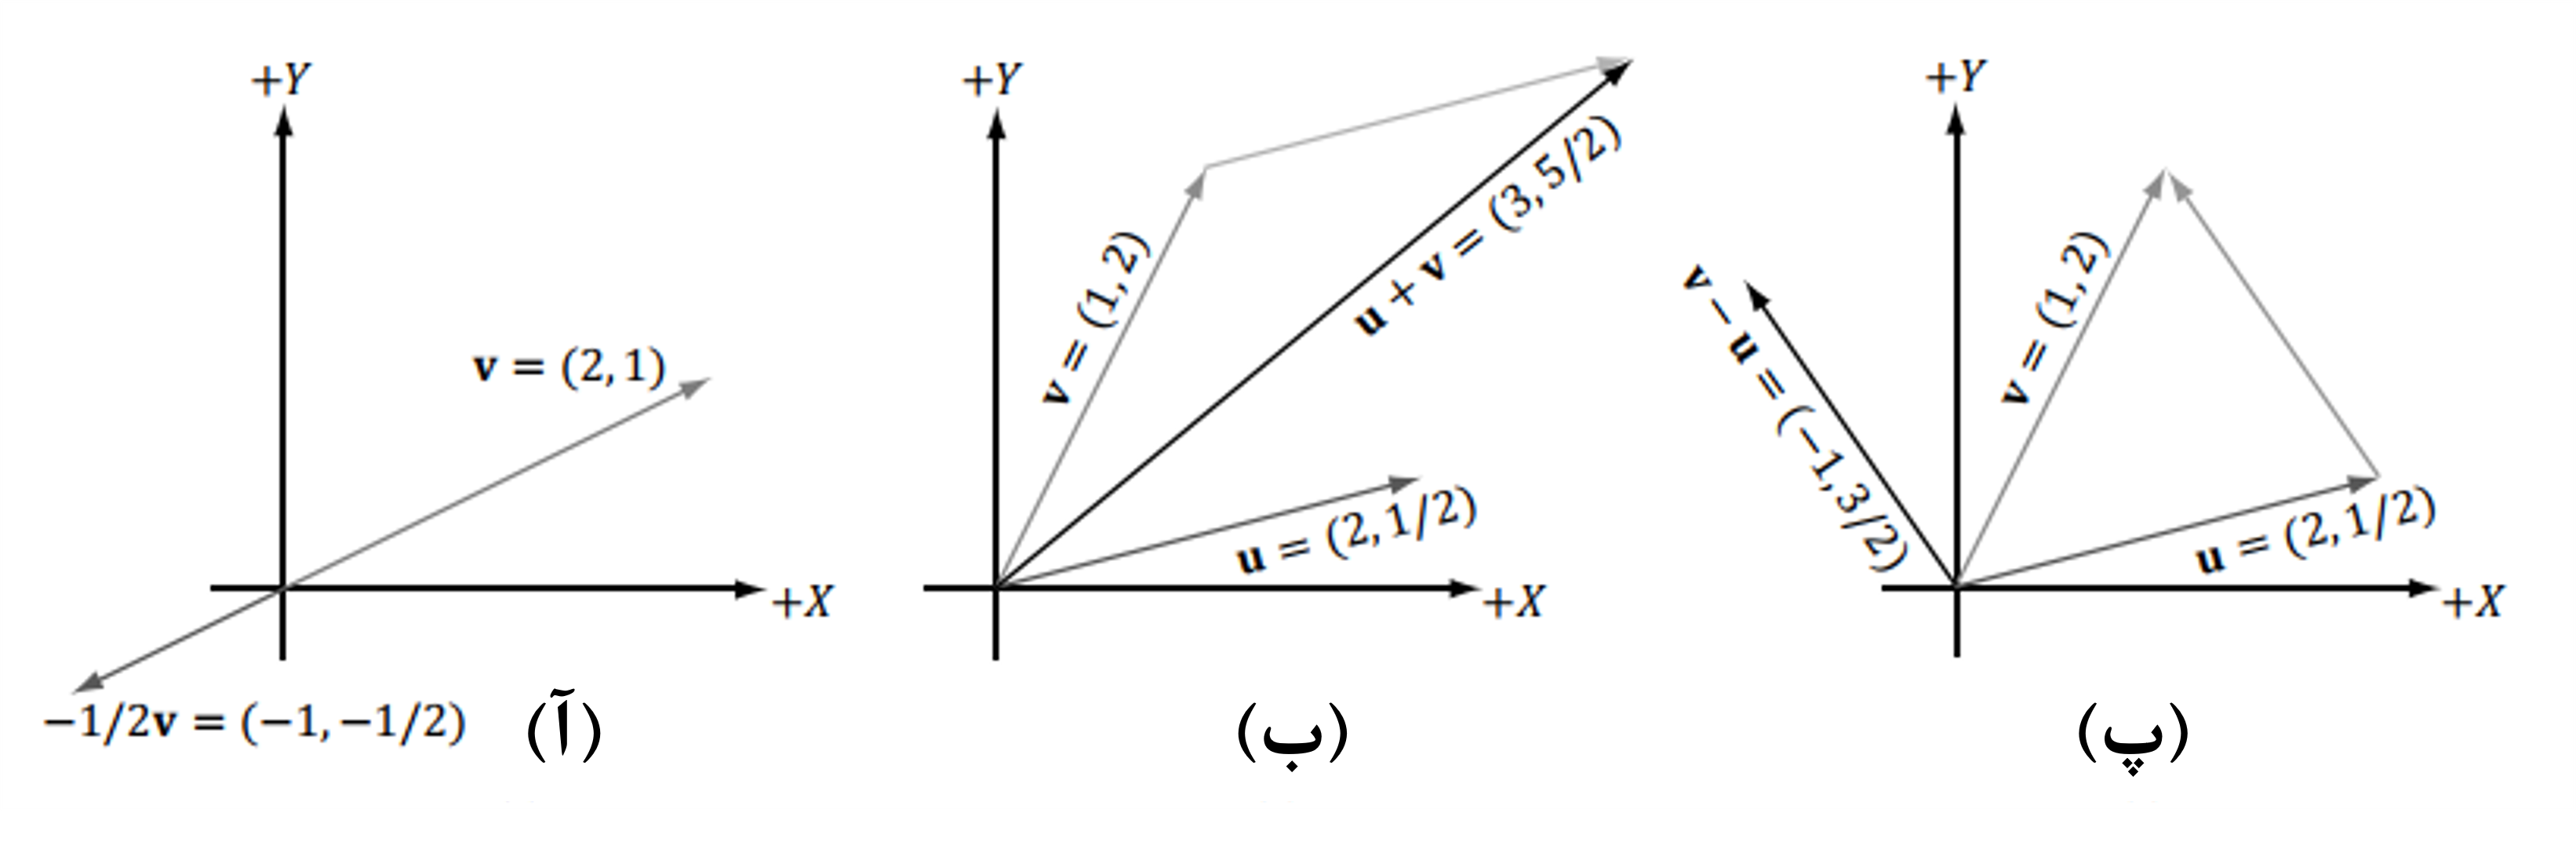
\includegraphics[width=\textwidth]{Images/4/4.Session.1.1.6}
            \caption{(آ) تفسیر هندسی ضرب اسکالر. (ب) تفسیر هندسی جمع بردار. ج) تفسیر هندسی تفریق بردار.}
            \label{fig:4.Session.1.1.6}
        \end{figure}

        \begin{figure}[H]
            \centering
            \setlength{\belowcaptionskip}{-10pt}
            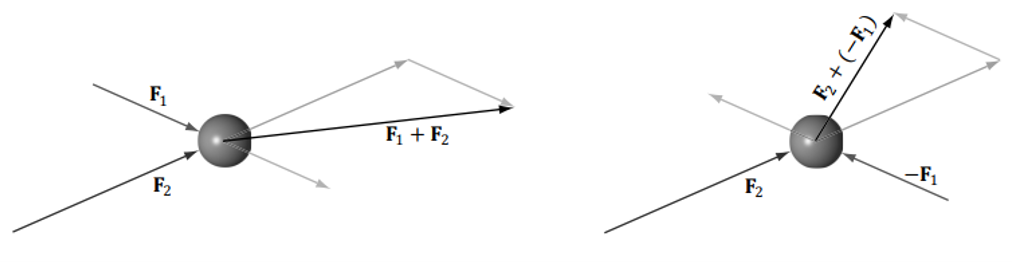
\includegraphics[width=\textwidth]{Images/4/4.Session.1.1.7}
            \caption{نیروهای اعمال شده به یک توپ. نیروها با استفاده از جمع بردار ترکیب می شوند تا نیروی برآیند به دست آید.}
            \label{fig:4.Session.1.1.7}
        \end{figure}
    \end{spacing}
}

{
    \textbf{\BTitr بردارهای طول و واحد}

    \Large
    \begin{spacing}{1.5}
        از نظر هندسی اندازه ی یک بردار، طول پاره خطی جهت دار است.
        اندازه ی یک بردار را با خط های عمودی دوتایی نشان می دهیم
        (به عنوان مثال، $\norm{u}$ اندازه ی $\textbf{u}$ را نشان می دهد).
        حالا با توجه به بردار $\textbf{u}=(x,y,z)$، می‌خواهیم بزرگی آن را به صورت جبری محاسبه کنیم.
        اندازه ی یک بردار سه بعدی را می توان با دو بار اعمال قضیه فیثاغورث محاسبه کرد.
        شکل \ref{fig:4.Session.1.1.8} را ببینید. ابتدا، ما به مثلث در صفحه xz با اضلاع x، z و وتر a نگاه می کنیم.

        \begin{figure}[H]
            \centering
            \setlength{\belowcaptionskip}{-10pt}
            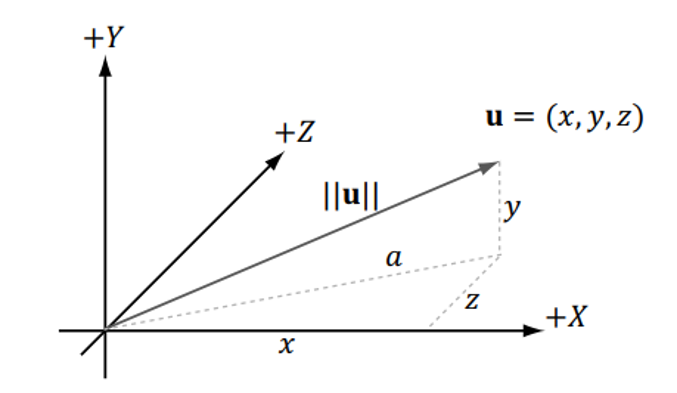
\includegraphics[width=0.5\textwidth]{Images/4/4.Session.1.1.8}
            \caption{طول سه بعدی یک بردار را می توان با دو بار اعمال قضیه فیثاغورث محاسبه کرد.}
            \label{fig:4.Session.1.1.8}
        \end{figure}

        از قضیه فیثاغورث، $a=\sqrt{\displaystyle x^2+z^2}$ داریم.
        حالا به مثلث با ضلع های \lr{a}، \lr{y} و وتر $\norm{u}$ نگاه کنید از قضیه فیثاغورث دوباره به فرمول اندازه ی زیر می رسیم:

        قضیه*****

        \begin{center}
            $\norm{\textbf{u}}=\sqrt{\displaystyle y^2+a^2}=\sqrt{\displaystyle y^2+(\sqrt{\displaystyle x^2+z^2})^2}=\sqrt{\displaystyle x^2+y^2+z^2}$
        \end{center}

        برای برخی از استفاده ها، ما به طول یک بردار اهمیتی نمی دهیم زیرا می خواهیم از بردار برای نمایش یک جهت خالص استفاده کنیم.
        می خواهیم طول چنین بردارهایی با فقط یک جهت دقیقاً 1 باشد.
        وقتی طول واحد برداری را می سازیم، می گوییم که بردار را نرمال کرده ایم.
        می توانیم یک بردار را با تقسیم هر یک از اجزای بر بزرگی آن ، نرمال کنیم:

        قضیه*****

        \begin{center}
            $\hat{\textbf{u}}=\frac{\displaystyle\textbf{u}}{\displaystyle\norm{\textbf{u}}}=\left(\frac{\displaystyle x}{\displaystyle\norm{\textbf{u}}},
            \frac{\displaystyle y}{\displaystyle\norm{\textbf{u}}}, \frac{\displaystyle z}{\displaystyle\norm{\textbf{u}}}\right)$
        \end{center}

        برای تأیید صحت این فرمول، می توانیم طول $\hat{\textbf{u}}$ را محاسبه کنیم

        \begin{center}
            $\norm{\hat{\textbf{u}}}=\sqrt{\left(\frac{\displaystyle x}{\displaystyle\norm{\textbf{u}}}\right)^2,
                \left(\frac{\displaystyle y}{\displaystyle\norm{\textbf{u}}}\right)^2,
                \left(\frac{\displaystyle z}{\displaystyle\norm{\textbf{u}}}\right)^2}=\frac{\displaystyle x^2+y^2+z^2}{\displaystyle\sqrt{\norm{\textbf{u}}^2}}
            =\frac{\displaystyle\norm{\textbf{u}}}{\displaystyle\norm{\textbf{u}}}=1$
        \end{center}


        پس \hat{\textbf{u}} در واقع یک بردار واحد است.

        مثال***

        بردار $\textbf{v}=(-1,3,4)$ را نرمال کنید. داریم $\norm{\textbf{v}}=\sqrt{\displaystyle (-1)^2+3^2+4^2}=\sqrt{26}$. پس:

        \begin{center}
            $\hat{\textbf{v}}=\frac{\displaystyle\textbf{v}}{\displaystyle\norm{\textbf{v}}}=\left(-\frac{\displaystyle 1}{\displaystyle\sqrt{26}},
            \frac{\displaystyle 3}{\displaystyle\sqrt{26}}, \frac{\displaystyle 4}{\displaystyle\sqrt{26}}\right)$
        \end{center}

        برای تأیید اینکه $\hat{\textbf{v}}$ واقعاً یک بردار واحد است، طول آن را محاسبه می کنیم:

        \begin{center}
            $\norm{\hat{\textbf{v}}}=\sqrt{\left(-\frac{\displaystyle 1}{\displaystyle\sqrt{26}}\right)^2,
                \left(\frac{\displaystyle 3}{\displaystyle\sqrt{26}}\right)^2, \left(\frac{\displaystyle 4}{\displaystyle\sqrt{26}}\right)^2}=
            \sqrt{\displaystyle\frac{\displaystyle 1}{\displaystyle 26}+\frac{\displaystyle 9}{\displaystyle 26}+\frac{\displaystyle 16}{\displaystyle 26}}=\sqrt{\displaystyle 1}=1$
        \end{center}

    \end{spacing}
}